\documentclass{article}

\usepackage{tikz}
	\usetikzlibrary{positioning,fit,calc, decorations, arrows, shapes, shapes.geometric}
	\usetikzlibrary{cd}

	%%%%%%%%%%%%
	\tikzset{AmpRep/.style={ampersand replacement=\&}}
	\tikzset{center base/.style={baseline={([yshift=-.8ex]current bounding box.center)}}}
	\tikzset{paperfig/.style={center base,scale=0.9, every node/.style={transform shape}}}

	% Node Stylings
	\tikzset{dpadded/.style={rounded corners=2, inner sep=0.7em, draw, outer sep=0.3em, fill={black!50}, fill opacity=0.08, text opacity=1}}
	\tikzset{dpad0/.style={outer sep=0.05em, inner sep=0.3em, draw=gray!75, rounded corners=4, fill=black!08, fill opacity=1, align=center}}
	\tikzset{dpad/.style args={#1}{every matrix/.append style={nodes={dpadded, #1}}}}
	\tikzset{light pad/.style={outer sep=0.2em, inner sep=0.5em, draw=gray!50}}
	
	
	\newcommand\cmergearr[5][]{
		\draw[arr, #1, -] (#2) -- (#5) -- (#3);
		\draw[arr, shorten <=0, #1] (#5) -- (#4);
	}
	\newcommand\mergearr[4][]{
		\coordinate (center-#2#3#4) at (barycentric cs:#2=1,#3=1,#4=1.2);
		\cmergearr[#1]{#2}{#3}{#4}{center-#2#3#4}
	}
	\newcommand\cunmergearr[5][]{
		\draw[arr, #1, -, shorten >=0] (#2) -- (#5);
		\draw[arr, shorten <=0, #1] (#5) -- (#3);
		\draw[arr, shorten <=0, #1] (#5) -- (#4);
	}
	\newcommand\unmergearr[4][]{
		\coordinate (center-#2#3#4) at (barycentric cs:#2=1.2,#3=1,#4=1);
		\cunmergearr[#1]{#2}{#3}{#4}{center-#2#3#4}
	}
	
	\newcommand\lab[1]{(#1)(lab-#1)}
	\tikzset{alternative/.style args={#1|#2|#3}{name=#1, circle, fill, inner sep=1pt,label={[name={lab-#1},gray!30!black, inner sep=1pt]#3:\scriptsize #2}} }
	
	
	\tikzset{bpt/.style args={#1|#2}{alternative={#1|#2|above}} }
	\tikzset{tpt/.style args={#1|#2}{alternative={#1|#2|below}} }
	\tikzset{lpt/.style args={#1|#2}{alternative={#1|#2|left}} }
	\tikzset{rpt/.style args={#1|#2}{alternative={#1|#2|right}} }
	\tikzset{pt/.style args={#1}{alternative={#1|#1|above}} }
	
	\tikzset{mpt/.style args={#1|#2}{name=#1, circle, fill, inner sep=1pt,label={[name={lab-#1},gray]\scriptsize #2}} }
	\tikzset{pt/.style args={#1}{name=#1, circle, fill, inner sep=1pt,label={[name={lab-#1},gray]\scriptsize #1}} }

	\tikzset{Dom/.style args={#1[#2] (#3) around #4}{dpadded, name=#3, label={[name={lab-#3},align=center,label distance=-1.9em, shading = axis, top color=white, bottom color=black!04, #2]150:#1}, fit={ #4 }, inner sep=0.5em}}
	\tikzset{tDom/.style args={#1 (#2) around #3}{dpadded, name=#2, label={[name={lab-#2},align=center] #1}, fit={ #3 } }}
	\tikzset{bDom/.style args={#1 (#2) around #3}{dpadded, name=#2, label={[name={lab-#2},align=center]below:#1}, fit={ #3 } }}

	\tikzset{arr/.style={draw, ->, thick, shorten <=3pt, shorten >=3pt}}
	\tikzset{arr0/.style={draw, ->, thick, shorten <=0pt, shorten >=0pt}}
	\tikzset{arr1/.style={draw, ->, thick, shorten <=1pt, shorten >=1pt}}
	\tikzset{arr2/.style={draw, ->, thick, shorten <=2pt, shorten >=2pt}}

\usepackage[utf8]{inputenc}
\usepackage{mathtools}
% \usepackage{bbold}
\usepackage{amssymb, graphicx}
\usepackage{parskip}
\usepackage{algorithm}
\usepackage{bbm}
\usepackage{faktor}
\usepackage{booktabs}
% \usepackage{algpseudocode}
\usepackage{graphicx}
\usepackage[margin=1.15in, marginpar=1.1in, marginparsep=14pt]{geometry}
\usepackage{scalerel}

\usepackage{hyperref} % Load before theorems...


\usepackage{enumitem}
\usepackage{amsthm,thmtools}
	\usepackage[noabbrev,nameinlink,capitalize]{cleveref}
    \theoremstyle{plain}
    \newtheorem{theorem}{Theorem}
	\newtheorem{coro}{Corollary}[theorem]
    \newtheorem{prop}[theorem]{Proposition}
    \newtheorem{claim}{Claim}
    \newtheorem{remark}{Remark}
    \newtheorem{lemma}[theorem]{Lemma}
    \theoremstyle{definition}
    \declaretheorem[name=Definition, qed=$\square$]{defn}

	\crefname{defn}{Definition}{Definitions}
	\crefname{prop}{Proposition}{Propositions}

\usepackage{nicefrac}\let\nf\nicefrac
\usepackage{color}
%\usepackage{stmaryrd}
\hypersetup{colorlinks=true, linkcolor=blue!75!black, urlcolor=magenta, citecolor=green!50!black}

\relax %%%%%%%%% GENERALL MACROS %%%%%%%%
    \let\Horig\H
	\let\H\relax
	\DeclareMathOperator{\H}{\mathrm{H}} % Entropy
	\DeclareMathOperator{\I}{\mathrm{I}} % Information
	\DeclareMathOperator*{\Ex}{\mathbb{E}} % Expectation

    \newcommand{\mat}[1]{\mathbf{#1}}
    \DeclarePairedDelimiterX{\infdivx}[2]{(}{)}{%
		#1\;\delimsize\|\;#2%
	}
	\newcommand{\thickD}{I\mkern-8muD}
	\newcommand{\kldiv}{\thickD\infdivx}
	\newcommand{\tto}{\rightarrow\mathrel{\mspace{-15mu}}\rightarrow}

	\newcommand{\datadist}[1]{\Pr\nolimits_{#1}}
	% \newcommand{\datadist}[1]{p_\text{data}}

	\makeatletter
	\newcommand{\subalign}[1]{%
	  \vcenter{%
	    \Let@ \restore@math@cr \default@tag
	    \baselineskip\fontdimen10 \scriptfont\tw@
	    \advance\baselineskip\fontdimen12 \scriptfont\tw@
	    \lineskip\thr@@\fontdimen8 \scriptfont\thr@@
	    \lineskiplimit\lineskip
	    \ialign{\hfil$\m@th\scriptstyle##$&$\m@th\scriptstyle{}##$\hfil\crcr
	      #1\crcr
	    }%
	  }%
	}
	\makeatother
	\newcommand\numberthis{\addtocounter{equation}{1}\tag{\theequation}}



\relax %%%%%%%%%   PDG  MACROS   %%%%%%%%
	\newcommand{\bp}[1][L]{\mat{p}_{\!_{#1}\!}}
	\newcommand{\bP}[1][L]{\mat{P}_{\!_{#1}\!}}
	\newcommand{\V}{\mathcal V}
	\newcommand{\N}{\mathcal N}
	\newcommand{\Ed}{\mathcal E}

	\DeclareMathAlphabet{\mathdcal}{U}{dutchcal}{m}{n}
	\DeclareMathAlphabet{\mathbdcal}{U}{dutchcal}{b}{n}
	\newcommand{\dg}[1]{\mathbdcal{#1}}
	\newcommand{\PDGof}[1]{{\dg M}_{#1}}
	\newcommand{\UPDGof}[1]{{\dg N}_{#1}}
	\newcommand\GFE{\mathit{G\mkern-4mu F\mkern-4.5mu E}}

	\newcommand\Inc{\mathit{Inc}}
	\newcommand{\IDef}[1]{\mathit{IDef}_{\!#1}}
	\newcommand{\ed}[3]{%
		\mathchoice%
		{#2\overset{\smash{\mskip-5mu\raisebox{-3pt}{${#1}$}}}{\xrightarrow{\hphantom{\scriptstyle {#1}}}} #3} %display style
		{#2\overset{\smash{\mskip-5mu\raisebox{-3pt}{$\scriptstyle {#1}$}}}{\xrightarrow{\hphantom{\scriptstyle {#1}}}} #3}% text style
		{#2\overset{\smash{\mskip-5mu\raisebox{-3pt}{$\scriptscriptstyle {#1}$}}}{\xrightarrow{\hphantom{\scriptscriptstyle {#1}}}} #3} %script style
		{#2\overset{\smash{\mskip-5mu\raisebox{-3pt}{$\scriptscriptstyle {#1}$}}}{\xrightarrow{\hphantom{\scriptscriptstyle {#1}}}} #3}} %scriptscriptstyle

    \newcommand{\nhphantom}[2]{\sbox0{\kern-2%
		\nulldelimiterspace$\left.\delimsize#1\vphantom{#2}\right.$}\hspace{-.97\wd0}}
		% \nulldelimiterspace$\left.\delimsize#1%
		% \vrule depth\dp#2 height \ht#2 width0pt\right.$}\hspace{-.97\wd0}}
	\makeatletter
	\newsavebox{\abcmycontentbox}
	\newcommand\DeclareDoubleDelim[5]{
	    \DeclarePairedDelimiterXPP{#1}[1]%
			{% box must be saved in this pre code
				\sbox{\abcmycontentbox}{\ensuremath{##1}}%
			}{#2}{#5}{}%
		    %%% Correct spacing, but doesn't work with externalize.
			% {\nhphantom{#3}{##1}\hspace{1.2pt}\delimsize#3\mathopen{}##1\mathclose{}\delimsize#4\hspace{1.2pt}\nhphantom{#4}{##1}}
			%%% Fast, but wrong spacing.
			% {\nhphantom{#3}{~}\hspace{1.2pt}\delimsize#3\mathopen{}##1\mathclose{}\delimsize#4\hspace{1.2pt}\nhphantom{#4}{~}}
			%%% with savebox.
		    {%
				\nhphantom{#3}{\usebox\abcmycontentbox}%
				\hspace{1.2pt} \delimsize#3%
				\mathopen{}\usebox{\abcmycontentbox}\mathclose{}%
				\delimsize#4\hspace{1.2pt}%
				\nhphantom{#4}{\usebox\abcmycontentbox}%
			}%
	}
	\makeatother
	\DeclareDoubleDelim
		\SD\{\{\}\}
	\DeclareDoubleDelim
		\bbr[[]]
	% \DeclareDoubleDelim
	% 	\aar\langle\langle\rangle\rangle
	\makeatletter
	\newsavebox{\aar@content}
	\newcommand\aar{\@ifstar\aar@one@star\aar@plain}
	\newcommand\aar@one@star{\@ifstar\aar@resize{\aar@plain*}}
	\newcommand\aar@resize[1]{\sbox{\aar@content}{#1}\scaleleftright[3.8ex]
		{\Biggl\langle\!\!\!\!\Biggl\langle}{\usebox{\aar@content}}
		{\Biggr\rangle\!\!\!\!\Biggr\rangle}}
	\DeclareDoubleDelim
		\aar@plain\langle\langle\rangle\rangle
	\makeatother


	% \DeclarePairedDelimiterX{\aar}[1]{\langle}{\rangle}
	% 	{\nhphantom{\langle}{#1}\hspace{1.2pt}\delimsize\langle\mathopen{}#1\mathclose{}\delimsize\rangle\hspace{1.2pt}\nhphantom{\rangle}{#1}}


%%%%% restatables and links
% \usepackage{xstring} % for expandarg
\usepackage{xpatch}
\makeatletter
\xpatchcmd{\thmt@restatable}% Edit \thmt@restatable
   {\csname #2\@xa\endcsname\ifx\@nx#1\@nx\else[{#1}]\fi}% Replace this code
   % {\ifthmt@thisistheone\csname #2\@xa\endcsname\typeout{oiii[#1;#2\@xa;#3;\csname thmt@stored@#3\endcsname]}\ifx\@nx#1\@nx\else[#1]\fi\else\csname #2\@xa\endcsname\fi}% with this code
   {\ifthmt@thisistheone\csname #2\@xa\endcsname\ifx\@nx#1\@nx\else[{#1}]\fi
   \else\fi}
   {}{\typeout{FIRST PATCH TO THM RESTATE FAILED}} % execute on success/failure
\xpatchcmd{\thmt@restatable}% A second edit to \thmt@restatable
   {\csname end#2\endcsname}
   {\ifthmt@thisistheone\csname end#2\endcsname\else\fi}
   {}{\typeout{FAILED SECOND THMT RESTATE PATCH}}

% \def\onlyaftercolon#1:#2{#2}
\newcommand{\recall}[1]{\medskip\par\noindent{\bf \Cref{thmt@@#1}.} \begingroup\em \noindent
   \expandafter\csname#1\endcsname* \endgroup\par\smallskip}
\newenvironment{linked}[3][]{%
	\def\linkedproof{#3}%
	\def\linkedtype{#2}%
	% \reversemarginpar
	% \marginpar{%
	% \vspace{1.1em}
	% % \hspace{2em}
	% 	% \raggedleft
	% 	\raggedright
	% 	\hyperref[proof:\linkedproof]{%
	% 	\color{blue!50!white}
	% 	\scaleleftright{$\Big[$}{\,{\small\raggedleft\tt\begin{tabular}{@{}c@{}} proof of \\\linkedtype~\ref*{\linkedtype:\linkedproof}\end{tabular}}\,}{$\Big]$}}
	% 	}%
	\restatable[#1]{#2}{#2:#3}\label{#2:#3}}
	{\endrestatable%
	% \par%\vspace{-0.5em}
	% \normalmarginpar
	\marginpar{%
		\vspace{-3em}
	% \hspace{2em}
		\raggedright
		\hyperref[proof:\linkedproof]{%
		\color{blue!50!white}
		\scaleleftright{$\Big[$}{\,{\small\raggedright\tt\begin{tabular}{@{}c@{}}
			% proof of \\\,\linkedtype~\ref*{\linkedtype:\linkedproof}
			link to\\
			proof
		\end{tabular}}\,}{$\Big]$}}
		}%
	}
\makeatother
	\newcounter{proofcntr}
	\newenvironment{lproof}{\begin{proof}\refstepcounter{proofcntr}}{\end{proof}}

	\usepackage[framemethod=TikZ]{mdframed}
	% \surroundwithmdframed[ % lproof
	% 	   topline=false,
	% 	   linewidth=3pt,
	% 	   linecolor=gray!20!white,
	% 	   rightline=false,
	% 	   bottomline=false,
	% 	   leftmargin=0pt,
	% 	   % innerleftmargin=5pt,
	% 	   skipabove=\medskipamount,
	% 	   skipbelow=\medskipamount
	% 	]{lproof}
%oli16: The extra space was because there was extra space in the paragraph, not
%because this length was too big. By breaking arrays, everything will be better.
\newcommand{\begthm}[3][]{\begin{#2}[{name=#1},restate=#3,label=#3]}

\title{}
\author{}
\date{May 2021}

%\allowdisplaybreaks

\begin{document}
	\section{Partial CPDs}
	Suppose we want to encode only part of a cpd. Suppose $A, B$ are variables, and we want to say that if $A$ takes a particular value $a^*$, then $B$ is distributed according to some distribution $p(B)$.
	This is a little bit like the usual cpd that we would attach to an edge $A \to B$---it is a conditional belief on $B$ given $A$---but only for one particular value of $A$. By contrast, to supply a cpd $p(B | A)$ for such an edge, you would need to give a distribution on $B$ for \emph{all} values of $A$.
	It turns out that the PDG formalism, without modification, is still expressive to allow you to specify this kind of information, with a little bit of extra structure which does not affect the semantics.

	Concretely, let's return to our example: we want to articulate a belief that $B \sim p$ if $A = a^*$, and say nothing otherwise.  We do this by introducing an auxiliary variable $X$, that can take a special value indicating that $A = a^*$, or any value of $B$. Now, supposing that $X$ takes the special value if and only if $A=a^*$, and otherwise takes the value of $B$, then there's a clear choice of distribution on $B$ given $X$: if $X$ takes its special value, we $\Pr(B) = p$. Otherwise, $\Pr(B)$ is a point mass on the value $b$. And this value of $X$ an be calculated from joint values of $B$ and $A$.  This PDG is illustrated below, with $\V(B) = \{b_1, b_1, \ldots b_n\}$.

	\begin{center}
		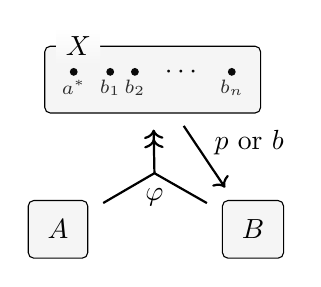
\begin{tikzpicture}[center base]
			\node[dpadded] (A) at (0,-0.5){$A$};
			\node[dpadded, right=1.5 of A](B){$B$};

			\node[tpt={astar|$a^*$}] at (0.2,1.5) {};
			\node[tpt={b1|$b_1$},right=0.35 of astar]{};
			\node[tpt={b2|$b_2$},right=0.2 of b1]{};
			\node[right=0.2 of b2] (bdots){$\cdots$};
			\node[tpt={bn|$b_n$},right=0.2 of bdots]{};

			\node[Dom={$X$[label distance=-2em, xshift=-1.0em] (X)
				around {\lab{astar}\lab{b1}\lab{bn}(1,1.65)}} ] {};


			\mergearr[->>]{A}{B}{X}
			\node[below=2pt of center-ABX]{$\varphi$};

			\draw[arr2] (X) to node[above right,yshift=-3pt]{$p$ or $b$} (B);
		\end{tikzpicture}
		\hspace{1cm}
		\begin{minipage}{0.3\textwidth}
			\begin{align*}
				\varphi(A,B) &:= \begin{cases}
					\delta_{X=a^*} & \text{if $A = a^*$} \\
					\delta_{X=B} & \text{otherwise}
				\end{cases}\\[1em]
				p \mathrm{~or~} b~(X) &:= \begin{cases}
					p(B) & \text{if $X = a^*$} \\
					\delta_{B=b} & \text{if $X = b$}
				\end{cases}
			\end{align*}

		\end{minipage}
	\end{center}
	\medskip

		This construction works because of the cycle, which in some sense peeks at the future to see the value of $B$ just in case $A \ne a^*$ and we don't want to indicate anything about the probability distribution on $B$. We now formalize the way in which it ``works'', semantically.


		\begin{prop}[Semantics work appropriately]
			\label{prop:sem1}
		Let $\dg M$ be the PDG above.
		\begin{enumerate}
			\item
				A distribution $\mu(A,B)$ shares marginals on $A$ and $B$ with some distribution $\mu(A,B,X)$ consistent with $\dg M$ if and only if $\mu(B \mid A = a^*) = p$.
%				 That is,
%				\[ \Big\{ \mu(A,B) ~\Big|~ \mu(A,B,X) \in \SD{\dg M}\Big\} =
%					\Big\{\mu(A,B) ~\Big|~ \mu(B\mid A \!=\! a^*) = p \Big\} .\]
			\item The incompatibility of $\dg M$ with a distribution $\mu(A,B,X)$ that satisfies $\varphi$ is the just the expected diveregence between $B$ and $\mu$ when $A = a^*$. It is also the incompatibility of $\mu$ with the PDG $A \xrightarrow{q} B$ where $q(B|A = a^*) = p$ and $q(B \mid A = a'\ne a^*) = \mu(B\mid a')$, and is given explicitly by
				\[ \Inc_{\dg M}(\mu:\Delta(ABX)) = \begin{cases}
					+\infty& \text{if~}\mu(X \ne \varphi(A,B)) >0 \\
					\Ex_\mu \Big[ \mathbbm1[{A\!=\!a^*}]  \kldiv{\mu(B\mid A\!=\!a^*)}{p} \Big] & \text{~otherwise.}
				\end{cases} \]

			\item $\IDef{\dg M}(\mu)$ is the $\mu$-expected-surprise in discovering that either $A= a^*$ (if it occurs), or the full sample $(a,b)$ if $A \ne a^*$. That is,
				\[ \IDef{\dg M}(\mu) =  \mu(A = a^*) \I_\mu[A = a^*] + \mu(A \ne A^*) \H(\mu \mid A = a^*). \]

			\item Regarding the PDG as a categorical diagram, its limit is the set consisting of $(a^*)$ and joint samples $(a,b)$ for $a \ne a$.  That is,
			\[ \lim \dg M = \{(a,b) : a \ne a^*, b \in B\} \cup \{ (a^*) \} \]
		\end{enumerate}
	\end{prop}
	\medskip
	\clearpage
	\section{Guard Variables}

	We now show how to build a similar widget for a guard, not unlike the widget used to compile hypergraphs to PDGs with regular edges. This time, let's consider the scenario where there's a third, binary variable $G$ representing a guard, and you have a cpd $p(B \mid A) $ which you only believe if the guard is true. We can represent this with a similar widget.

	\begin{center}
		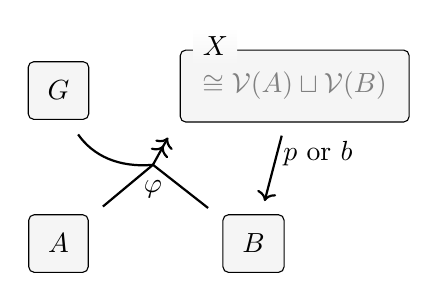
\begin{tikzpicture}[center base]
			\node[dpadded] (A) at (0,-0.5){$A$};
			\node[dpadded, right=1.5 of A](B){$B$};
			\node[dpadded, above=1 of A](G){$G$};

%			\node[dpadded, inner sep=0.8em, label={[label distance=-1.5em,shading = axis, top color=white, bottom color=black!04, xshift=2.2em]145:$G\,{?}A\,{:}\,B$}, text=gray] (GAB) at (3,1.5) {$\cong \V(A) \sqcup \V(B)$};
			\node[dpadded, inner sep=0.8em, label={[label distance=-1.5em,shading = axis, top color=white, bottom color=black!04, xshift=-1.0em]145:$X$}, text=gray] (GAB) at (3,1.5) {$\cong \V(A) \sqcup \V(B)$};
%

%			\mergearr[->>]{A}{B}{GAB}
			\coordinate (cent) at (1.2, 0.5);
			\draw[arr,-] (A) -- (cent) to[] (B);
			\draw[arr,->>] (G) to[bend right] (cent) -- (GAB.south west);
%			\node[below=2pt of cent]{$G\,{?}A\,{:}\,B$};
			\node[below=2pt of cent]{$\varphi$};

			\draw[arr2] (GAB) to node[above right,yshift=-3pt]{$p$ or $b$} (B);
		\end{tikzpicture}
		\hspace{1cm}
		\begin{minipage}{0.3\textwidth}
			\begin{align*}
				\varphi(G,A,B) &:= \text{ if } G \text{ then } A \text{ else } B. \\[1em]
				p \mathrm{~or~} b~(X) &:= \begin{cases}
					p(B|A\!=\!a) & \text{if } X = a \\
					\delta_{B=b} & \text{if } X = b \\
				\end{cases}
			\end{align*}

		\end{minipage}
	\end{center}

	With this widget, we can make all knowledge conditional, and

	\begin{prop}
		Semantic properties analogous to \Cref{prop:sem1} hold for guard variables.
	\end{prop}
	\begin{prop}
		A widget encoding a guard variable $G$ for a link $A \to B$, together with a belief $(\to G)$ that the guard is always true, is semantically equivalent to the original link $A \to B$, without a guard.
	\end{prop}

\end{document}
